% Contenuto di "143_capitoli/capitolo2/immagini_capitolo_2/grafo_squared.tex"
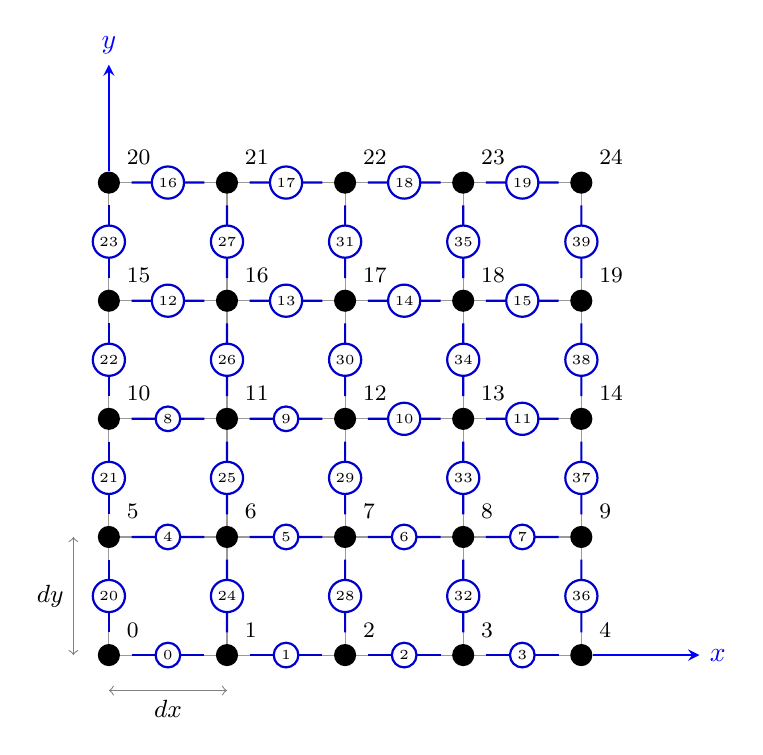
\begin{tikzpicture}[
    scale=1.5, 
    punto/.style={circle, fill=black, inner sep=0pt, minimum size=8pt}, 
    fune/.style={draw=blue!80!black, thick, shorten >=4pt, shorten <=4pt}, 
    asse/.style={->, >=stealth, blue, thick},
    el_oriz/.style={circle, draw=blue!80!black, fill=white, font=\tiny\color{black}, inner sep=1.5pt},
    el_vert/.style={circle, draw=blue!80!black, fill=white, font=\tiny\color{black}, inner sep=1.5pt},
    every label/.style={font=\footnotesize, black} 
]

    % 1. Assi cartesiani
    \draw[asse] (4.1,0) -- (5.0,0) node[right] {$x$};
    \draw[asse] (0,4.1) -- (0, 5.0) node[above] {$y$};
    
    % LA GRIGLIA DI SFONDO
    % Disegna una griglia dal punto (0,0) al punto (4,4) con passo 1.0 (coincidente con i nodi)
    \draw[gray!80, thin, step = 1.0] (0,0) grid (4,4);
    
    % Quote passi dx e dy
    \draw[<->, gray] (0,-0.3) -- (1,-0.3) node[midway, below, black] {\small $dx$};
    \draw[<->, gray] (-0.3,0) -- (-0.3,1) node[midway, left, black] {\small $dy$};

    % 2. Definizione dei Nodi (25 nodi totali, matrice 5x5, nx = 5)
    % Riga y = 0
    \node[punto, label={45:0}] (N0) at (0,0) {};
    \node[punto, label={45:1}] (N1) at (1,0) {};
    \node[punto, label={45:2}] (N2) at (2,0) {};
    \node[punto, label={45:3}] (N3) at (3,0) {};
    \node[punto, label={45:4}] (N4) at (4,0) {};
    
    % Riga y = 1
    \node[punto, label={45:5}] (N5) at (0,1) {};
    \node[punto, label={45:6}] (N6) at (1,1) {};
    \node[punto, label={45:7}] (N7) at (2,1) {};
    \node[punto, label={45:8}] (N8) at (3,1) {};
    \node[punto, label={45:9}] (N9) at (4,1) {};
    
    % Riga y = 2
    \node[punto, label={45:10}] (N10) at (0,2) {};
    \node[punto, label={45:11}] (N11) at (1,2) {};
    \node[punto, label={45:12}] (N12) at (2,2) {};
    \node[punto, label={45:13}] (N13) at (3,2) {};
    \node[punto, label={45:14}] (N14) at (4,2) {};
    
    % Riga y = 3
    \node[punto, label={45:15}] (N15) at (0,3) {};
    \node[punto, label={45:16}] (N16) at (1,3) {};
    \node[punto, label={45:17}] (N17) at (2,3) {};
    \node[punto, label={45:18}] (N18) at (3,3) {};
    \node[punto, label={45:19}] (N19) at (4,3) {};
    
    % Riga y = 4
    \node[punto, label={45:20}] (N20) at (0,4) {};
    \node[punto, label={45:21}] (N21) at (1,4) {};
    \node[punto, label={45:22}] (N22) at (2,4) {};
    \node[punto, label={45:23}] (N23) at (3,4) {};
    \node[punto, label={45:24}] (N24) at (4,4) {};

    % 3. Elementi Orizzontali (20 elementi, numeri da 0 a 19 cerchiati sulla fune)
    % y = 0
    \draw[fune] (N0) -- (N1) node[midway, el_oriz] {0};
    \draw[fune] (N1) -- (N2) node[midway, el_oriz] {1};
    \draw[fune] (N2) -- (N3) node[midway, el_oriz] {2};
    \draw[fune] (N3) -- (N4) node[midway, el_oriz] {3};
    
    % y = 1
    \draw[fune] (N5) -- (N6) node[midway, el_oriz] {4};
    \draw[fune] (N6) -- (N7) node[midway, el_oriz] {5};
    \draw[fune] (N7) -- (N8) node[midway, el_oriz] {6};
    \draw[fune] (N8) -- (N9) node[midway, el_oriz] {7};
    
    % y = 2
    \draw[fune] (N10) -- (N11) node[midway, el_oriz] {8};
    \draw[fune] (N11) -- (N12) node[midway, el_oriz] {9};
    \draw[fune] (N12) -- (N13) node[midway, el_oriz] {10};
    \draw[fune] (N13) -- (N14) node[midway, el_oriz] {11};
    
    % y = 3
    \draw[fune] (N15) -- (N16) node[midway, el_oriz] {12};
    \draw[fune] (N16) -- (N17) node[midway, el_oriz] {13};
    \draw[fune] (N17) -- (N18) node[midway, el_oriz] {14};
    \draw[fune] (N18) -- (N19) node[midway, el_oriz] {15};
    
    % y = 4
    \draw[fune] (N20) -- (N21) node[midway, el_oriz] {16};
    \draw[fune] (N21) -- (N22) node[midway, el_oriz] {17};
    \draw[fune] (N22) -- (N23) node[midway, el_oriz] {18};
    \draw[fune] (N23) -- (N24) node[midway, el_oriz] {19};

    % 4. Elementi Verticali (20 elementi, numeri da 20 a 39 cerchiati sulla fune)
    % x = 0
    \draw[fune] (N0) -- (N5) node[midway, el_vert] {20};
    \draw[fune] (N5) -- (N10) node[midway, el_vert] {21};
    \draw[fune] (N10) -- (N15) node[midway, el_vert] {22};
    \draw[fune] (N15) -- (N20) node[midway, el_vert] {23};
    
    % x = 1
    \draw[fune] (N1) -- (N6) node[midway, el_vert] {24};
    \draw[fune] (N6) -- (N11) node[midway, el_vert] {25};
    \draw[fune] (N11) -- (N16) node[midway, el_vert] {26};
    \draw[fune] (N16) -- (N21) node[midway, el_vert] {27};
    
    % x = 2
    \draw[fune] (N2) -- (N7) node[midway, el_vert] {28};
    \draw[fune] (N7) -- (N12) node[midway, el_vert] {29};
    \draw[fune] (N12) -- (N17) node[midway, el_vert] {30};
    \draw[fune] (N17) -- (N22) node[midway, el_vert] {31};
    
    % x = 3
    \draw[fune] (N3) -- (N8) node[midway, el_vert] {32};
    \draw[fune] (N8) -- (N13) node[midway, el_vert] {33};
    \draw[fune] (N13) -- (N18) node[midway, el_vert] {34};
    \draw[fune] (N18) -- (N23) node[midway, el_vert] {35};
    
    % x = 4
    \draw[fune] (N4) -- (N9) node[midway, el_vert] {36};
    \draw[fune] (N9) -- (N14) node[midway, el_vert] {37};
    \draw[fune] (N14) -- (N19) node[midway, el_vert] {38};
    \draw[fune] (N19) -- (N24) node[midway, el_vert] {39};

\end{tikzpicture}